% Chapter 3

\chapter{Results} % Main chapter title

\label{Chapter3} % For referencing the chapter elsewhere, use \ref{Chapter1} 

\lhead{Chapter 3. \emph{Computational experimentation}} % This is for the header on each page - perhaps a shortened title

%----------------------------------------------------------------------------------------

Nowadays scientific computing is one the most important tools for scientific discovery. Computational implementation became crucial when the problem cannot be solved by traditional experimental or theoretical means. There are a number or reasons why this might happen, for example whenever experimentation may be dangerous, to expensive or time-consuming.

Stochastic topology has embraced the methods of scientific computing to provide a better insight of complex phenomena. A lot of techniques has been used in this sense, for example, the use of algorithms that sample the search space.

For theoretical develop it has allowed to verify if the established conditions in a probabilistic model are sharp enough, meaning that a random object satisfy certain property  so that the model describe desire properties or if the conjectures on certain properties are valid or not \cite{Meshulam13}.

In this work we propose to generate random graphs for the Ërdos Renyi model using \textbf{python}

\section{Simulating graphs in G(n,p)}
 To simulate graphs in this model we can notice that the information of the graph is summarized in its adyacency matrix. If the graph has $n$ vertices then the we'll have a matriz of size $n \times n$, where the entry $a_{i,j}$ it's equal to 1 if the vertex $i$ and the vertex $j$ are connected, and it's $0$ otherwise. As we are considering simple no-directed graphs, this matrix is symetric with zeros in the diagonal. Thus it's enough to simulate each entry above the diagonal with a r.v. $Bernoulli(p)$.

WE can directly do the implementation of this simulation can be find in the function: \texttt{erdosRenyi}. Usying the libary \href{https://networkx.github.io/}{NetworkX} we can create and modify graphs directly taken grpahs as objects in python.

In the figure \ref{fig:ErdosRenyi10} we can see a set of graphs obtained with such algorithm, fixing $n=10$ an varing the parameter $p$
\begin{figure}[h!]
	\centering
	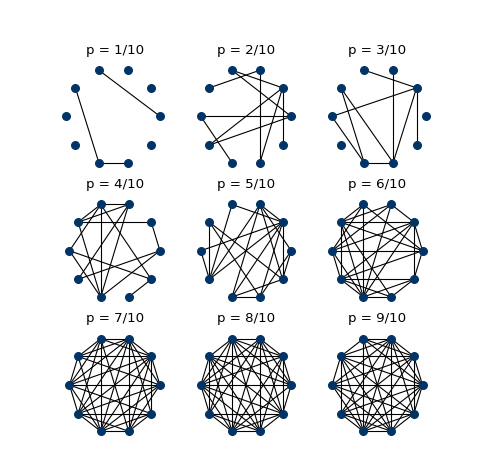
\includegraphics[scale=1]{Figures/ER-10.png}
	\caption{Erdös-Rényi random graphs with $n$ fixed and varing $p$}
	\label{fig:ErdosRenyi10}
\end{figure}

As we mention in the introduction the utility of doing Como se menciona en la introducción la utilidad de las simulaciones para el desarrollo de la topología estocástica reside en poder verificar la rigurosidad de las condiciones impuestas para que cierta propiedad se satisfaga, en este caso la propiedad es la conexidad y las condiciones están dadas por la cota $log(n)/n$ para $p$. Para ejemplificar esto se hicieron simulaciones en Python de gráficas variando $n$ y tomando $p$ como indica el teorema con $\omega(n)= log(n/2)$. Para cada tamaño de $n$ se repite la simulación 30 veces y se verifica si la gráfica simulada es conexa o no con la función \texttt{is$\_$connected(G)} de la librería de \texttt{networkX}. De esta manera obtenemos una aproximación de la probabilidad de que una gráfica sea conexa si se toma con las condiciones indicadas en el teorema. En la figura \ref{fig:Estimadas}, se graficó para cada $n$ dicha probabilidad estimada para cada caso de $p$.

\begin{figure}[h!]
	\centering
	\includegraphics[scale=0.8]{estimadas.png}
	\caption{Probabilidad estimada de conexidad para distintas gráficas tomando el parámetro p como se indica en el teorema}
	\label{fig:Estimadas}
\end{figure}

Analizando la figura \ref{fig:Estimadas} es fácil convencerse de la validez del teorema viendo que para $n$ suficientemente grande $n=50$, la gráfica muestra lo establecido en el teorema.

La ejecución del algoritmo erdosRenyi implementado requiere de la generación de $\binom{n}{2}$ variables aleatorias Bernoulli las cuales son simuladas en el código de Python adjunto en la función \texttt{Bernoulli}, las cuales hacen uso de la librería de \texttt{numpy} para generar los números aleatorios básicos, librería que usa el algoritmo \textbf{Mersenne-Twister}. Por lo que el tiempo de ejecución del algoritmo es de $O(n^{2})$. En la figura \ref{fig:tiemposER} se muestran los resultados de los tiempos de ejecución haciendo variar $n$.

\begin{figure}[h!]
	\centering
	\includegraphics[scale=0.8]{tiemposER.png}
	\caption{Tiempos de ejecución en segundos del algoritmo erdosRenyi variando el tamaño de la gráfica. Se presenta la escala norma y la logarítmica}
	\label{fig:tiemposER}
\end{figure}



\section{The algorithm}
The aim of this section is to discuss the computational difficulties of implementing an algorithm which produces rigid expansions on a graph $G$, starting from a subset $A$. We'll be taking about the algorithm regardless of whether the optimizations and considerations appear in the context of the graph of curves. Then by the end of the chapter we'll fit the results to the context that we described in the pasts chapters. The purpose to do it so, is because the combinatorial nature of the phenomena make sense by it self, even more in the stochastic point of view we're considering a non-monothonous process.

A priori, the algorithm to determine a first rigid expansion it's supposed to be executed in a large amount of time, as the definition let us see, it depends not only on the size of $G$, it also depends on the size of $A$; it's necessarily to seek among all the possible subsets of $A$ that's $2^{m}$ verifications where $|A| = m$. This tells us that if we are going to be dealing with large stochastic graphs it's important to do some optimization to the algorithms and see when does this have more impact in the expected execution time according to the taken parameters.

Any isolated vertex in $A$ wont have any impact at the moment of doing rigid expansions, so they shouldn't be consider, also whenever leaves appear in the set it's convenient to ignore them. Unique neighbors of leaves which we will call \textit{petioles} should be automatically added to set because of the definition of a single rigid expansion.

It means that we are now working with the set:
$$A' = A - \{v: deg(v)\leq 1 \} \cup \{u: \exists x, N(x)=\{u\}\} $$

